\documentclass{beamer}
\usepackage{graphicx}
\usepackage{amsmath, amsthm, amsfonts, amssymb, mathrsfs, mathtools}
\usepackage{textcomp} % straigth apos
\usepackage{tikz}
\usepackage{verbatim}
\usepackage{tikzit}
\usepackage{listings}
\usepackage{subfig}
\usepackage[ruled,vlined, linesnumbered]{algorithm2e}
\usepackage{algorithmic,float}


\input{graphs.tikzstyles}

% \usefonttheme{serif}

\theoremstyle{definition}

\setbeamercovered{invisible}

\setbeamertemplate{theorems}[numbered]
\setbeamertemplate{lemma}[numbered]
\newtheorem{remark}{Remark}

\newcommand{\xra}[1]{\overset{#1}{\rightsquigarrow}}

\usetheme{Madrid}
\useoutertheme{tree} % Alternatively: miniframes, infolines, split
\useinnertheme{circles}


\setbeamertemplate{headline}
{%
  \leavevmode%
  \begin{beamercolorbox}[wd=.5\paperwidth,ht=2.5ex,dp=1.125ex]{section in head/foot}%
    \hbox to .5\paperwidth{\hfil\insertsectionhead\hfil}
  \end{beamercolorbox}%
  \begin{beamercolorbox}[wd=.5\paperwidth,ht=2.5ex,dp=1.125ex]{subsection in head/foot}%
    \hbox to .5\paperwidth{\hfil\insertsubsectionhead\hfil}
  \end{beamercolorbox}%
}

\setbeamertemplate{section in toc}{%
  \inserttocsectionnumber.~\inserttocsection}
\setbeamercolor{section in toc}{fg=black}
\setbeamercolor{subsection in toc}{fg=structure}
\setbeamertemplate{subsection in toc}{%
  \hspace{1.2em}{\tiny\inserttocsectionnumber.\inserttocsubsectionnumber}~\small\inserttocsubsection\par}

% \setbeamertemplate{bibliography item}{\insertbiblabel.~\insertbibitem}

\definecolor{lightbrown}{RGB}{207, 161, 118}

\usecolortheme[named=lightbrown]{structure}

\title[Model Checking Real-Time Systems]{Model Checking Real-Time Systems}
\date{December 12, 2022}
\author[V. Trélat]{Vincent Trélat}
\institute[TUM]{Technical University of Munich}

\begin{document}

\begin{frame}
\titlepage
\end{frame}

\begin{frame}
\tableofcontents
\end{frame}

\section{Timed Automata}
\subsection{Preliminaries}

\begin{frame}
  \tableofcontents[currentsection]
\end{frame}

\begin{frame}
  Set of \emph{time values}: $\mathbb{R}_{\geq 0}$
  \vfill
  \emph{Timed words} over $\Sigma \times \mathbb{R}_{\geq 0}$
  \vfill
  Set of \emph{valuations} over a set of clocks $C$: $\mathbb{R}_{\geq 0}^C$
  \vfill
  \emph{Constraints} over $C$: $\varphi ::= x \odot k\ |\ \varphi \land \varphi$ where $x \in C$, $k \in \mathbb{Z}$ and $\odot \in \{<, \leq, =, \geq, >\}$
  \vfill
  Set of valuations \emph{satisfying} $\varphi$: $[\![\varphi]\!]_C = \{v \in \mathbb{R}_{\geq 0}^C\ |\ v \models \varphi\}$
\end{frame}


\subsection{Timed Automata}

\begin{frame}
  \begin{definition}
    A \emph{Timed Automaton} (TA) $\mathcal{A}$ is the tuple $(L, \ell_0, C, \Sigma, I, E)$ where:
    \begin{itemize}
      \item $L$ is a finite set of \emph{locations} with initial location $\ell_0 \in L$
      \item $C$ is a finite set of \emph{clocks}
      \item $\Sigma$ is a finite set of \emph{actions}
      \item $I \colon L \to \varPhi(C)$ is an \emph{invariant mapping}
      \item $E \subseteq L \times \varPhi(C) \times \Sigma \times 2^{C} \times L$ is a set of edges.
    \end{itemize}
  \end{definition}
  \vfill
  Edges are denoted by $\ell \xrightarrow{\varphi, a, r} \ell'$.
\end{frame}
\begin{frame}
  Example of a TA with 3 locations, 2 clocks and 2 actions (letters):
  \ctikzfig{ex_ta}
\end{frame}

\begin{frame}{Operational Semantics}
\onslide<1->{
\begin{figure}
  \centering
  \begin{tikzpicture}
  \small
	\begin{pgfonlayer}{nodelayer}
		\node [style=white, align=center] (0) at (-2, 0) {$\ell$ \\ $y \leq 1$};
		\node [style=white, align=center] (1) at (2, 0) {$\ell'$ \\ $y \leq 2$};
		\node [style=none] (2) at (0, -0.25) {$x > 1, x := 0$};
		\node [style=none] (3) at (0, 0.25) {$a$};
	\end{pgfonlayer}
	\begin{pgfonlayer}{edgelayer}
		\draw [->, thick] (0) -- (1);
	\end{pgfonlayer}
\end{tikzpicture}
\end{figure}
}
\onslide<2->{
  \begin{equation*}
    \begin{cases}
      v(x) = {\color{red}1.2}\\
      v(y) = {\color{red}0.8}
    \end{cases}
    \onslide<3->{
    \quad
    (\ell, v) \xrightarrow{{\color{red}0.5},\ a} (\ell', v')
    \quad
    }
    \onslide<4->{
    \begin{cases}
      v'(x) = {\color{red}0}\\
      v'(y) = {\color{red}1.3}
    \end{cases}
    }
  \end{equation*}
}
\end{frame}

\begin{frame}{Operational Semantics}
  \only<1>{
  \begin{figure}
    \centering
    \begin{tikzpicture}
    \small
    \begin{pgfonlayer}{nodelayer}
      \node [style=white, align=center] (0) at (-2, 0) {$\ell$ \\ $y \leq 1$};
      \node [style=white, align=center] (1) at (2, 0) {$\ell'$ \\ $y \leq 2$};
      \node [style=none] (2) at (0, -0.25) {$x > 1, x := 0$};
      \node [style=none] (3) at (0, 0.25) {$a$};
    \end{pgfonlayer}
    \begin{pgfonlayer}{edgelayer}
      \draw [->, thick] (0) -- (1);
    \end{pgfonlayer}
  \end{tikzpicture}
  \end{figure}
  }
  \only<2->{
  \begin{figure}
    \centering
    \begin{tikzpicture}
    \small
    \begin{pgfonlayer}{nodelayer}
      \node [style=white, align=center] (0) at (-2, 0) {$\ell$ \\ $\ I(\ell)\ $};
      \node [style=white, align=center] (1) at (2, 0) {$\ell'$ \\ $\ I(\ell')\ $};
      \node [style=none] (2) at (0, -0.25) {$\varphi, r$};
      \node [style=none] (3) at (0, 0.25) {$a$};
    \end{pgfonlayer}
    \begin{pgfonlayer}{edgelayer}
      \draw [->, thick] (0) -- (1);
    \end{pgfonlayer}
  \end{tikzpicture}
  \end{figure}
  }
  \only<3>{
  \begin{equation*}
    (\ell, v) \xrightarrow{d,\ a} (\ell', v')
  \end{equation*}
  }
  \only<4->{
  \begin{equation*}
    (\ell, v) \xrightarrow{d,\ a} (\ell', (v+d)[r])
  \end{equation*}
  }
  \onslide<5->{
  provided that:
  $$\ell \xrightarrow{\varphi, a, r} \ell'\ \text{is a transition in the TA}$$
  $$\forall t \in [0, d], \ v + t \models I(\ell)$$
  $$v + d \models I(\ell')$$
  }
\end{frame}

\begin{frame}
  \frametitle{Operational Semantics}
\begin{definition}
  \small
  The \emph{operational semantics} of a TA $A = (L, \ell_0, C, \Sigma, I, E)$ is the infinite-state timed transition system $[\![A]\!] = (S, s_0, \Sigma \times \mathbb{R}_{\geq 0}, T)$, where
  \begin{align*}
	  &S := \{(\ell, v) \in L \times \mathbb{R}_{\geq 0}^C\ |\ v \models I(\ell)\}, \quad s_0 := (\ell_0, \text{\bf 0}_C),\\
	  &T := \{(\ell, v) \xrightarrow{d, a} (\ell', (v+d)[r]) \ | \ d \in \mathbb{R}_{\geq 0}, \\
    &\quad\quad\quad\quad\forall d' \in [0, d], v + d' \models I(\ell) \land \exists \ell \xrightarrow{\varphi, a, r} \ell' \in E, v + d \models \varphi \}
  \end{align*}
\end{definition}
\end{frame}

\subsection{Regions and zones}

\begin{frame}
  \tableofcontents[currentsection, currentsubsection]
\end{frame}

\begin{frame}{Region Equivalence}
  \onslide<1->{
  \begin{definition}
  \small
  Two valuations $v, v' \in \mathbb{R}_{\geq 0}^C$ are region equivalent, i.e\ $v \cong_M v'$ iff:
  \begin{itemize}
    \item $\forall x \in C, \lfloor v(x) \rfloor = \lfloor v'(x) \rfloor \ \lor \ v(x), v'(x) > M_x$
    \item $\forall x \in C, \langle v(x) \rangle = 0 \Leftrightarrow \langle v'(x) \rangle = 0 \ \lor \ v(x) \geq M_x$
    \item $\forall x, y \in C, \langle v(x) \rangle \leq \langle v(y) \rangle \Leftrightarrow \langle v'(x) \rangle \leq \langle v'(y) \rangle \ \lor \ v(x) > M_x \ \lor \ v(y) > M_y$
  \end{itemize}
\end{definition}
  }
  \onslide<2->{
    \begin{center}
      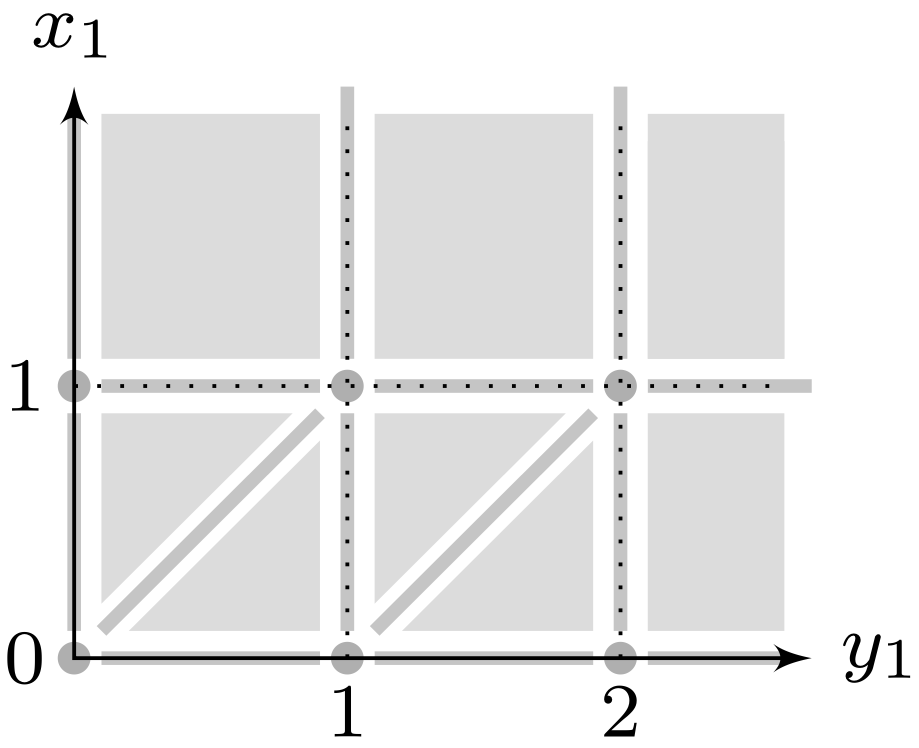
\includegraphics[height=10em]{../img/TAreg.png}
    \end{center}
  }
\end{frame}

\begin{frame}
\begin{definition}[Region Automaton]
  $\mathcal{R}_{\cong_M}(A) = (S, s_0, \Sigma, T)$ is the \emph{region automaton} of $A$, where:
  \begin{itemize}
    \item $S := (L \times \mathbb{R}_{\geq 0}^C)_{/\cong_M},\ s_0 := \text{\bf 0}_C$
    \item $T := \{[\ell, v]_{\cong_M} \xrightarrow{a} [\ell', v']_{\cong_M}\ |\ \exists d \in \mathbb{R}_{\geq 0}, (\ell, v) \xrightarrow{d, a} (\ell', v')\}$
  \end{itemize}
\end{definition}
\begin{itemize}
  \item<2> $\left| S \right|$ is exponential in the number of clocks and in the maximal constants of the timed automaton
  \item<2> Is there a way to reduce the number of states?
\end{itemize}
\end{frame}

\begin{frame}
  \begin{definition}[Zone]
    A set of valuations $Z \subseteq \mathbb{R}_{\geq 0}^C$ is a zone iff:
    $\exists \varphi \in \varPhi_d(C), Z = [\![\varphi]\!]_C$
    
    In this case, we define:
    \begin{itemize}
      \item the \emph{delay} of $Z$: $Z^\uparrow \triangleq \{ v + d \ |\ V \in Z \land d \in \mathbb{R}_{\geq 0}\}$
      \item the \emph{reset} of $Z$: $Z[r] \triangleq \{ v[r] \ |\ v \in Z\}$ for $r \subseteq C$
    \end{itemize}
  \end{definition}
  \small
  \begin{definition}[Zone automaton]
    The \emph{zone automaton} $[\![A]\!]_Z$ of $A$ is the tuple $(S, s_0, \Sigma \cup \{\delta\}, T)$, where:\\
      $$S := \{ (\ell, Z)\ |\ \ell \in L, Z \in \mathbb{R}_{\geq 0}^C\ \text{is a zone}\},\quad s_0 := (\ell_0, [\![\text{\bf 0}_C]\!])$$
    \begin{align*}
      &T := \{ (\ell, Z) \xra{\delta} (\ell', Z^\uparrow \cap [\![I(\ell)]\!]_C)\} \cup \\
      &\{ (\ell, Z) \xra{a} (\ell', (Z \cap [\![I(\ell)]\!]_C)[r] \cap [\![I(\ell')]\!]_C) \ |\ \ell \xrightarrow{\varphi, a, r} \ell' \in E\}
    \end{align*}
  \end{definition}
\end{frame}

\subsection{Extensions}

\section{Model Checking Real-Time Systems}
\subsection{TLTL}
\subsection{Timed Games}

\section{Language-Theoretic Properties}

\section{References}
\begin{frame}{References}
  \setbeamertemplate{bibliography item}{\insertbiblabel}
  \bibliographystyle{abbrv}
  \bibliography{../abstract/ref}
\end{frame}

\end{document}